\documentclass[11pt,preprint]{elsarticle}

\usepackage{lmodern}
%%%% My spacing
\usepackage{setspace}
\setstretch{1.2}
\DeclareMathSizes{12}{14}{10}{10}

% Wrap around which gives all figures included the [H] command, or places it "here". This can be tedious to code in Rmarkdown.
\usepackage{float}
\let\origfigure\figure
\let\endorigfigure\endfigure
\renewenvironment{figure}[1][2] {
    \expandafter\origfigure\expandafter[H]
} {
    \endorigfigure
}

\let\origtable\table
\let\endorigtable\endtable
\renewenvironment{table}[1][2] {
    \expandafter\origtable\expandafter[H]
} {
    \endorigtable
}


\usepackage{ifxetex,ifluatex}
\usepackage{fixltx2e} % provides \textsubscript
\ifnum 0\ifxetex 1\fi\ifluatex 1\fi=0 % if pdftex
  \usepackage[T1]{fontenc}
  \usepackage[utf8]{inputenc}
\else % if luatex or xelatex
  \ifxetex
    \usepackage{mathspec}
    \usepackage{xltxtra,xunicode}
  \else
    \usepackage{fontspec}
  \fi
  \defaultfontfeatures{Mapping=tex-text,Scale=MatchLowercase}
  \newcommand{\euro}{€}
\fi

\usepackage{amssymb, amsmath, amsthm, amsfonts}

\def\bibsection{\section*{References}} %%% Make "References" appear before bibliography


\usepackage[numbers]{natbib}

\usepackage{longtable}
\usepackage[margin=2.3cm,bottom=2cm,top=2.5cm, includefoot]{geometry}
\usepackage{fancyhdr}
\usepackage[bottom, hang, flushmargin]{footmisc}
\usepackage{graphicx}
\numberwithin{equation}{section}
\numberwithin{figure}{section}
\numberwithin{table}{section}
\setlength{\parindent}{0cm}
\setlength{\parskip}{1.3ex plus 0.5ex minus 0.3ex}
\usepackage{textcomp}
\renewcommand{\headrulewidth}{0.2pt}
\renewcommand{\footrulewidth}{0.3pt}

\usepackage{array}
\newcolumntype{x}[1]{>{\centering\arraybackslash\hspace{0pt}}p{#1}}

%%%%  Remove the "preprint submitted to" part. Don't worry about this either, it just looks better without it:
\makeatletter
\def\ps@pprintTitle{%
  \let\@oddhead\@empty
  \let\@evenhead\@empty
  \let\@oddfoot\@empty
  \let\@evenfoot\@oddfoot
}
\makeatother

 \def\tightlist{} % This allows for subbullets!

\usepackage{hyperref}
\hypersetup{breaklinks=true,
            bookmarks=true,
            colorlinks=true,
            citecolor=blue,
            urlcolor=blue,
            linkcolor=blue,
            pdfborder={0 0 0}}


% The following packages allow huxtable to work:
\usepackage{siunitx}
\usepackage{multirow}
\usepackage{hhline}
\usepackage{calc}
\usepackage{tabularx}
\usepackage{booktabs}
\usepackage{caption}


\newenvironment{columns}[1][]{}{}

\newenvironment{column}[1]{\begin{minipage}{#1}\ignorespaces}{%
\end{minipage}
\ifhmode\unskip\fi
\aftergroup\useignorespacesandallpars}

\def\useignorespacesandallpars#1\ignorespaces\fi{%
#1\fi\ignorespacesandallpars}

\makeatletter
\def\ignorespacesandallpars{%
  \@ifnextchar\par
    {\expandafter\ignorespacesandallpars\@gobble}%
    {}%
}
\makeatother


% definitions for citeproc citations
\NewDocumentCommand\citeproctext{}{}
\NewDocumentCommand\citeproc{mm}{%
\href{\#cite.\detokenize{#1}}{#2}\nocite{#1}}

\makeatletter
% allow citations to break across lines
\let\@cite@ofmt\@firstofone
% avoid brackets around text for \cite:
\def\@biblabel#1{}
\def\@cite#1#2{{#1\if@tempswa , #2\fi}}
\makeatother
\newlength{\cslhangindent}
\setlength{\cslhangindent}{1.5em}
\newlength{\csllabelwidth}
\setlength{\csllabelwidth}{3em}
\newenvironment{CSLReferences}[2] % #1 hanging-indent, #2 entry-spacing
{\begin{list}{}{%
	\setlength{\itemindent}{0pt}
	\setlength{\leftmargin}{0pt}
	\setlength{\parsep}{0pt}
	% turn on hanging indent if param 1 is 1
	\ifodd #1
	\setlength{\leftmargin}{\cslhangindent}
	\setlength{\itemindent}{-1\cslhangindent}
	\fi
	% set entry spacing
	\setlength{\itemsep}{#2\baselineskip}}}
{\end{list}}

\usepackage{calc}
\newcommand{\CSLBlock}[1]{\hfill\break\parbox[t]{\linewidth}{\strut\ignorespaces#1\strut}}
\newcommand{\CSLLeftMargin}[1]{\parbox[t]{\csllabelwidth}{\strut#1\strut}}
\newcommand{\CSLRightInline}[1]{\parbox[t]{\linewidth - \csllabelwidth}{\strut#1\strut}}
\newcommand{\CSLIndent}[1]{\hspace{\cslhangindent}#1}


\urlstyle{same}  % don't use monospace font for urls
\setlength{\parindent}{0pt}
\setlength{\parskip}{6pt plus 2pt minus 1pt}
\setlength{\emergencystretch}{3em}  % prevent overfull lines
\setcounter{secnumdepth}{5}

%%% Use protect on footnotes to avoid problems with footnotes in titles
\let\rmarkdownfootnote\footnote%
\def\footnote{\protect\rmarkdownfootnote}
\IfFileExists{upquote.sty}{\usepackage{upquote}}{}

%%% Include extra packages specified by user
\usepackage{colortbl}
\usepackage{graphicx}
\usepackage{adjustbox}
\usepackage{framed}
\usepackage{fancyvrb}
\DefineVerbatimEnvironment{Shaded}{Verbatim}{frame=single}\usepackage{booktabs}
\usepackage{longtable}
\usepackage{array}
\usepackage{multirow}
\usepackage{wrapfig}
\usepackage{float}
\usepackage{colortbl}
\usepackage{pdflscape}
\usepackage{tabu}
\usepackage{threeparttable}
\usepackage{threeparttablex}
\usepackage[normalem]{ulem}
\usepackage{makecell}
\usepackage{xcolor}

%%% Hard setting column skips for reports - this ensures greater consistency and control over the length settings in the document.
%% page layout
%% paragraphs
\setlength{\baselineskip}{12pt plus 0pt minus 0pt}
\setlength{\parskip}{12pt plus 0pt minus 0pt}
\setlength{\parindent}{0pt plus 0pt minus 0pt}
%% floats
\setlength{\floatsep}{12pt plus 0 pt minus 0pt}
\setlength{\textfloatsep}{20pt plus 0pt minus 0pt}
\setlength{\intextsep}{14pt plus 0pt minus 0pt}
\setlength{\dbltextfloatsep}{20pt plus 0pt minus 0pt}
\setlength{\dblfloatsep}{14pt plus 0pt minus 0pt}
%% maths
\setlength{\abovedisplayskip}{12pt plus 0pt minus 0pt}
\setlength{\belowdisplayskip}{12pt plus 0pt minus 0pt}
%% lists
\setlength{\topsep}{10pt plus 0pt minus 0pt}
\setlength{\partopsep}{3pt plus 0pt minus 0pt}
\setlength{\itemsep}{5pt plus 0pt minus 0pt}
\setlength{\labelsep}{8mm plus 0mm minus 0mm}
\setlength{\parsep}{\the\parskip}
\setlength{\listparindent}{\the\parindent}
%% verbatim
\setlength{\fboxsep}{5pt plus 0pt minus 0pt}



\begin{document}



\begin{frontmatter}  %

\title{Baby Name Trend Analysis in the United States}

% Set to FALSE if wanting to remove title (for submission)




\author[Add1]{Marjella Ernst}
\ead{marjella.ernst@web.de}





\address[Add1]{Stellenbosch University, Stellenbosch, South Africa}



\vspace{1cm}





\vspace{0.5cm}

\end{frontmatter}

\setcounter{footnote}{0}



%________________________
% Header and Footers
%%%%%%%%%%%%%%%%%%%%%%%%%%%%%%%%%
\pagestyle{fancy}
\chead{}
\rhead{}
\lfoot{}
\rfoot{\footnotesize Page \thepage}
\lhead{}
%\rfoot{\footnotesize Page \thepage } % "e.g. Page 2"
\cfoot{}

%\setlength\headheight{30pt}
%%%%%%%%%%%%%%%%%%%%%%%%%%%%%%%%%
%________________________

\headsep 35pt % So that header does not go over title




\section{\texorpdfstring{Introduction
\label{Introduction}}{Introduction }}\label{introduction}

This report analyses trends in US baby names over the years 1910 until
2014. The analysis is supported by data on famous singers and actors
names in the same time period. In the course of the analysis,
persistence and volatility of name popularity are being explored over
time, to analyse whether names that are popular in a given year tend to
remain popular three years in the future.

To do this, I calculate and visualise the Spearman rank correlation for
the 25 most popular names in each year, comparing them to the top names
three years thereafter. This provides a measure of how stable or
fast-changing baby name trends have been and whether these trends have
become more volatile after 1990.

In addition, I investigate sudden surges in name popularity and
cross-reference these with publications in music and film. Specifically,
I cross-check, whether names have spiked in popularity following the
success of certain songs, singers, actresses or characters. By combining
name data with cultural references, the analysis aims to identify
potential drivers of naming trends and provide guidance for selecting
toy character names that have the potential to be liked by future baby
generations.

\section{Methodology}\label{methodology}

\subsection{Data Overview}\label{data-overview}

In a first step, data is loaded in from the data folder and stored in
variables.

Consequently, data is being checked for NAs and duplicates.

The baby names dataset comprises US baby names from 1910 to 2014, with
state-level observations differentiated by gender. In the next step, a
graph is being created, showing the total number of babys in the data
set over time, to get a feeling for the data. As shown in Figure
@ref(fig:name-count), the total number of recorded names demonstrates
significant variation over this 104-year period.

\begin{figure}[H]

{\centering 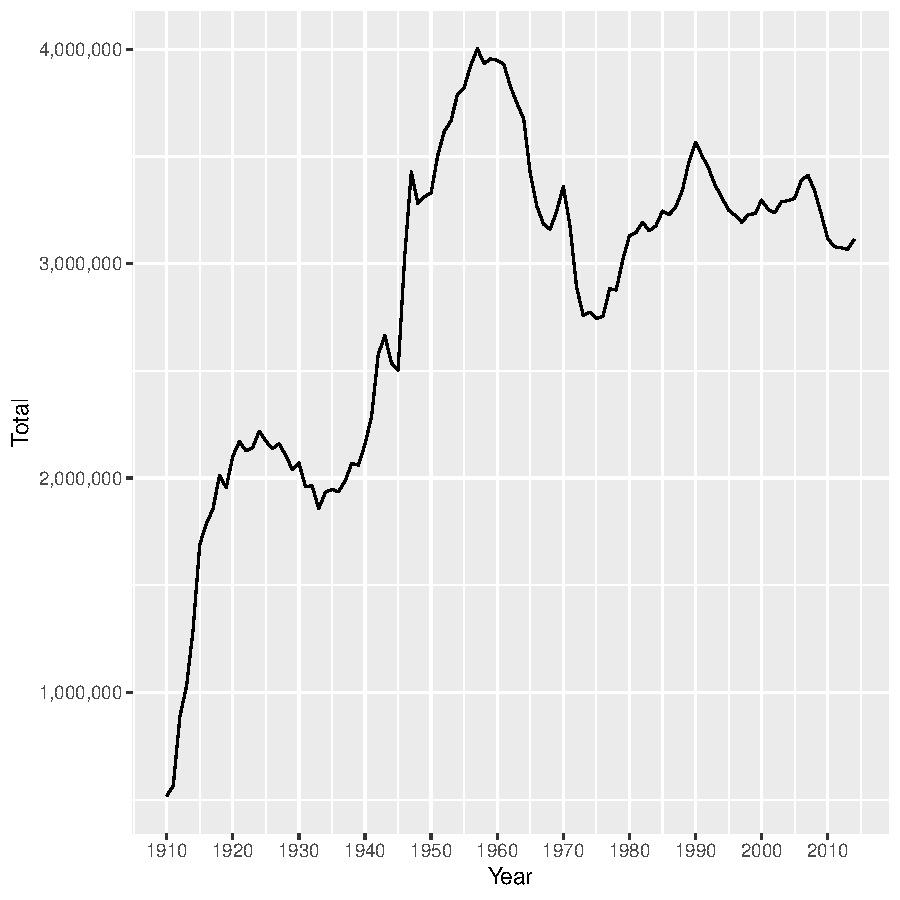
\includegraphics{Task_1_ReadMe_files/figure-latex/name-count-1} 

}

\caption{Annual Count of Unique Baby Names in the U.S., 1910-2014}\label{fig:name-count}
\end{figure}

\subsection{Analysis Steps}\label{analysis-steps}

The following chapter summarizes the results of the data analyses.

\subsection{Mainstream Analysis}\label{mainstream-analysis}

Now I carry out a ``mainstream analysis'' meaning I check how many
children had the most popular name of the year, differentiated between
male and female names.

\begin{figure}
\centering
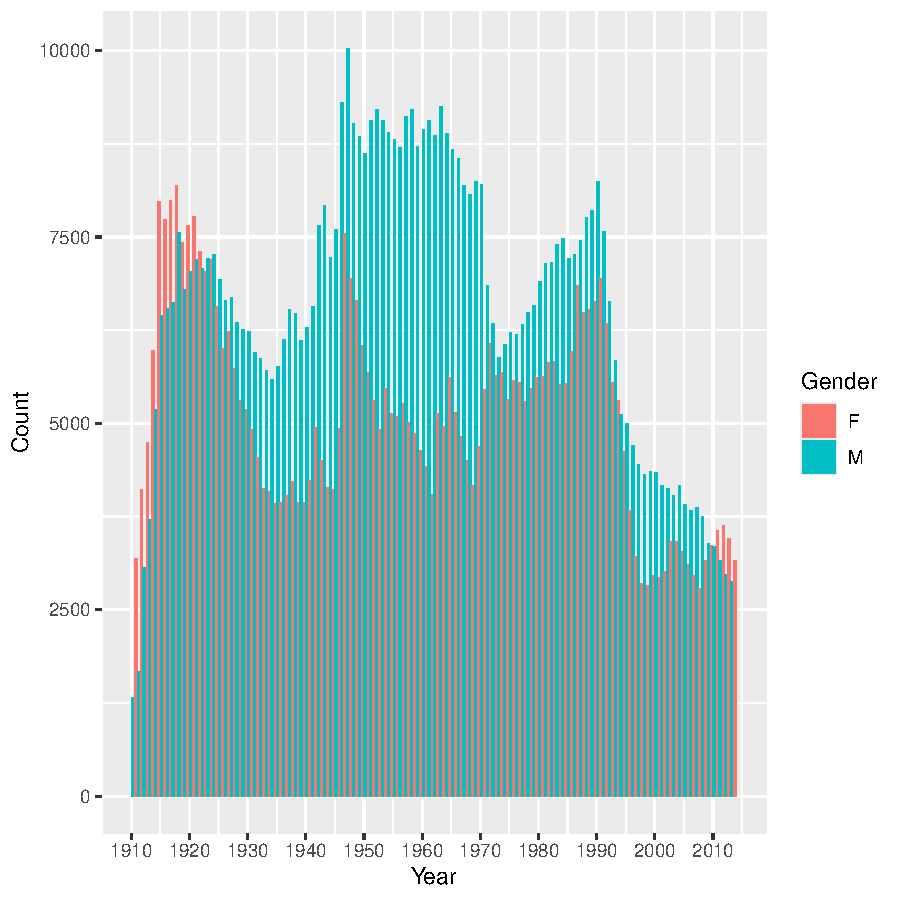
\includegraphics{Task_1_ReadMe_files/figure-latex/unnamed-chunk-3-1.pdf}
\caption{Mainstream Analysis}
\end{figure}

\subsection{Persistence Analysis}\label{persistence-analysis}

To analyse whether the persistency of names has changed over the time
horizon 1910 until 2011, a Spearmen Rank Correlation is being calculated
between top 25 names on the country-level in year t0 and t3. The period
had to be limited to 2011 as this is the last year for which the +3
years time lag can be calculated. The results of the persistency
analysis (Figure \textcite{ref}(fig:correlation)) suggests that
persistence of names follows a decreasing trend overall, indicating that
name preferences change faster today than they did in the mid 19th
century. Comparing the means of Spearmen rank correlation coefficients
before and after 1990 has confirms the hypothesis that popular names
persisted slower after 1990. The mean of correlation coefficients before
1990 amounts to 0.857, while the mean thereafter reduces to 0.766,
indicating faster-paced name trends.

\begin{figure}[H]

{\centering 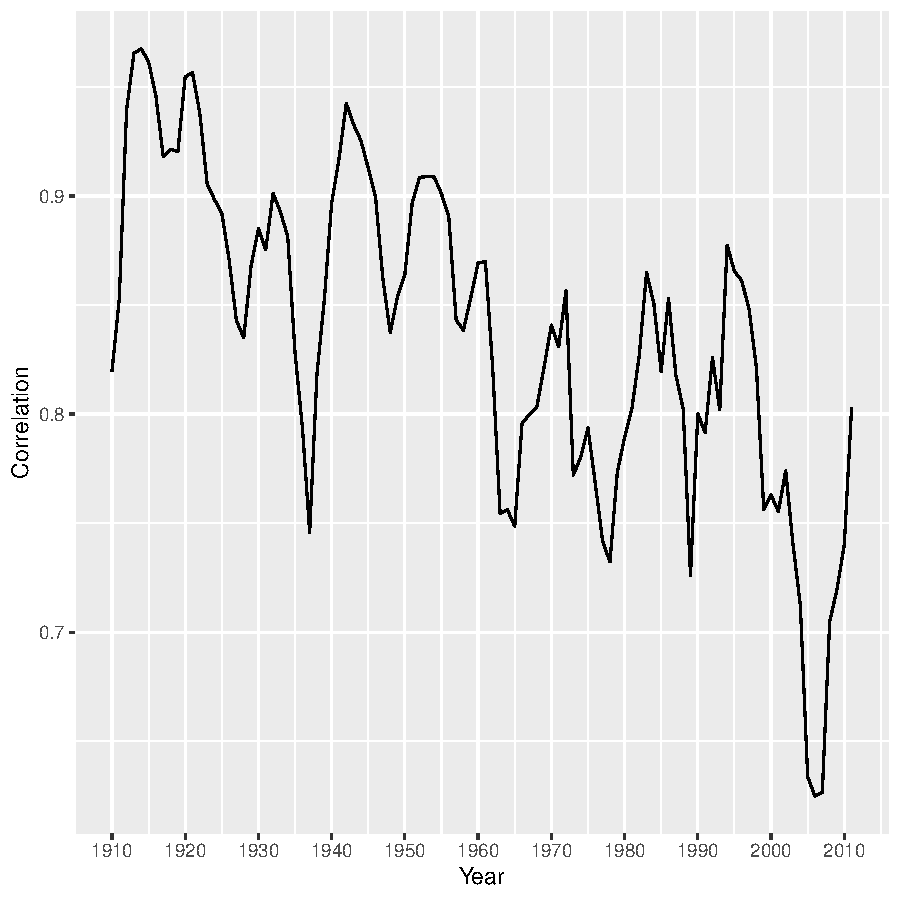
\includegraphics{Task_1_ReadMe_files/figure-latex/fig-correlation-1} 

}

\caption{Correlation Trend Over Time (1910–2011)}\label{fig:fig-correlation}
\end{figure}

However, after correlation reduced considerably between the 1990s and
early years of the present century, this trend has reversed after 2005.
In the year 2011, Spearmen correlation is only slightly lower that in
the beginning of the time series in 1910, indicating a recent shift
towards more higher persistence of names.

\subsection{Spike Analysis}\label{spike-analysis}

The spike analysis was carried out to test which names have experienced
the largest hypes in the period under analysis. @ref(tab:top-spikes)
displays the 15 mostly hyped names, as indicated by their percentage
increase in usage between two years. Interestingly, 12 out of the 15
names are female names, indicating names for baby girls are experiencing
more extreme hypes. It has also been analysed, whether these names
appear in movie or music productions. Surprisingly, out of these top 15
most spiked names, only the name Aja shows a relation to the film
industry. The next subchapter analyses the impact of film and music
publications on names overall.

\begin{longtable}[t]{rllr}
\caption{\label{tab:top-spikes}Top 15 Baby Name Spikes by Percentage Increase}\\
\toprule
Year & Name & Gender & \% Increase\\
\midrule
1964 & Deneen & F & 31340.0\\
1994 & Aaliyah & F & 28140.0\\
1983 & Mallory & F & 13060.0\\
2010 & Tenley & F & 12900.0\\
1957 & Tammie & F & 11580.0\\
\addlinespace
1992 & Jalen & M & 9616.7\\
1978 & Aja & F & 8620.0\\
2012 & Cataleya & F & 7600.0\\
1928 & Jeannine & F & 7440.0\\
1981 & Krystle & F & 6816.7\\
\addlinespace
1968 & Dustin & M & 6550.0\\
1995 & Lyric & F & 6320.0\\
1966 & Tabitha & F & 5960.0\\
2000 & Elian & M & 5922.2\\
2005 & Mikalah & F & 5680.0\\
\bottomrule
\end{longtable}

\subsection{Pop-Culture Analysis}\label{pop-culture-analysis}

Thereafter, billboard data is being used to check whether famous baby
names relate to music pop-culture. The music\_check function organizes
the billboard data by top 20 songs per year and checks whether artist or
song names relate to baby names. It then assigns two dummy columns to
the spikes data frame, telling us whether names appear in top 20 singer
or song names within the time frame 1910 until 2014.

A similar analysis is being done for the movie data stored in
hbo\_titles and hbo\_credits. In a first step, both data frames are
being merged based on the id column. Therafter, unnecessary columns are
deselected and only films with rating higher than 8.5 and published
before 2014 selected. Then, str\_detect() is being used to check whether
names occur in movie titles, character or actor names, or the movie
description. In a last step, a dummy column is being added to provide
information if the name is related to a popular movie.

In a last step, it is being analysed, how many names per gender are
related to famous singers, songs or movies. This analysis is insightful
to provide recommendations for the toy company, which elements of pop
culture to get toy name inspiration from.

\begin{table}
\centering
\caption{\label{tab:spikes}Name Representation in Pop Culture}
\centering
\begin{tabular}[t]{l|l|l|l}
\hline
Gender & pct\_artist & pct\_song & pct\_film\\
\hline
F & 8.4\% & 2.6\% & 16.1\%\\
\hline
M & 15.1\% & 3.5\% & 30.5\%\\
\hline
\end{tabular}
\end{table}

\section{Recommendations}\label{recommendations}

In a last step, names from actors or actresses of recent (as of 2014)
and highly rated movies (\textgreater{} viewer rating 8.5) are being
isolated to serve as source of inspiration for new toy names.
Movie-related names are being chosen as they were found to influence
baby name choice more than singer or song names.

\begin{longtable}[t]{l}
\caption{\label{tab:recommendations}Top Name Predictions}\\
\toprule
Names\\
\midrule
Angourie\\
Annie\\
Aya\\
Brene\\
Chukwudi\\
\addlinespace
Danielle\\
Evan\\
Guy\\
James\\
Janina\\
\addlinespace
Joe\\
Kenjiro\\
Kentaro\\
Marc\\
Mark\\
\addlinespace
Martha\\
Neal\\
Nobuyuki\\
Ramon\\
Yuma\\
\bottomrule
\end{longtable}

\section{Conclusion}\label{conclusion}

In conclusion, the analysis has provided evidence for the fact that baby
name trends have become more fast-paced over the course of the recent
decades. This is supported by the finding that mean correlation
coefficients before 1990 are higher than those after 1990. However, data
visualization in @ref(fig:correlation)) suggests a recent increase in
correlation coefficients, indicating a slow-down of the previous
fast-paced name trend development.

To analyse the sources of spikes in names over the years, billboard data
on famous singers and songs, as well as Hbo data on movies, movie
characters and actors has been analysed for their effect on name
popularity. The findings of this analysis suggest that film-related
names have had the largest effect on both male (30\%) and female names
(16\%), followed by artist names (5.8\% on female and 10.5\% on male
names). The lowest effect was found by song names, only contributing to
2.5\% of male and 1.7\% of female names.

These findings suggest that toy names should be inspired by movie
characters or actresses, as these are the major sources of inspiration
for baby names. Looking at recent film trends, possible candidates could
for instance be Mahershala, Ivana or Yuki.

\newpage

\bibliography{Tex/ref}





\end{document}
